% =====================================================================
% Milestone 2, paper-sized cut. Same text as paper/milestone2_short.md.
% Paste into the acmart main .tex. Needs \usepackage{booktabs}.
% Figure paths are relative to the repo root: upload the two PNGs to
% Overleaf under the same paths, or edit the paths.
% Add the two BibTeX entries at the bottom of this file to the .bib.
% =====================================================================

% ---------- Methodology insert (after the simulator paragraph) ----------

Our blackjack simulator uses six decks. The dealer stands on soft 17 and peeks
for blackjack, players may double on any two cards (including after a split),
one split is allowed, there is no surrender or insurance, and blackjack pays
3:2. The basic strategy for these rules comes from the Wizard of Odds chart
\cite{wizardofodds}. Its exact house edge is 0.457\% per hand, and a bot playing the chart lost 0.43\% per hand over three million simulated hands, consistent with the published edge for these rules. All results so
far use Qwen2.5-7B \cite{qwen2024qwen25}, 4-bit quantized and run locally
through Ollama at temperature 0. We evaluate the baseline two ways: a
\emph{natural run} of 1,000 dealt hands, and a \emph{scenario set} that forces
each of the 330 basic-strategy cells once so that rare hands count equally. As
a secondary metric, \emph{EV loss} is the expected value of the basic-strategy
action minus that of the chosen action, in units per one-unit bet.

% ---------- Results and Discussion ----------

\section{Results and Discussion}
\label{sec:results}

All results are for the baseline configuration, with every harness component
turned off. They are the reference point that each component will be measured
against on the identical seeded hands, the first step toward measuring how
much performance the harness adds beyond the model itself.

\begin{table}[t]
  \caption{Baseline results for Qwen2.5-7B with all harness components off.
  Brackets are Wilson 95\% confidence intervals.}
  \label{tab:main}
  \begin{tabular}{lll}
    \toprule
    Metric & Natural run (1,000 hands) & Scenario set (330 cells) \\
    \midrule
    Decisions graded & 1,147 & 330 \\
    \textbf{Decision accuracy} & \textbf{41.7\%} [38.9--44.6] & \textbf{40.9\%} [35.7--46.3] \\
    Accuracy: hard / soft / pair & 41.8 / 42.2 / 40.4\% & 38.7 / 33.8 / 50.0\% \\
    Invalid-action rate & 0.8\% & 2.7\% \\
    Mean return per hand & $-0.330$ units & --- (forced hands) \\
    EV loss per decision & 0.328 units & 0.266 units \\
    \bottomrule
  \end{tabular}
\end{table}

\subsection{Decision Accuracy}

The baseline matched basic strategy on 41.7\% of decisions in the natural run
and on 40.9\% of scenario cells (Table~\ref{tab:main}). The natural run is
dominated by common hard totals, while the scenario set weights every cell
equally, but the two confidence intervals overlap almost entirely. So the
model's errors are not concentrated in rare hands. They are spread across the
whole strategy table. The natural run lost 0.330 units per hand, compared with
0.457\% for perfect basic strategy. At 1,000 hands that return is too noisy to
interpret on its own, so decision accuracy remains the primary metric.

\subsection{Systematic Over-Doubling}

The dominant error is doubling. Basic strategy doubles on 9.7\% of natural-run
decisions, but the model doubled on 41.2\%. Meanwhile it hit on only 17.2\% of
decisions, where basic strategy hits on 40.9\%. The doubling is poorly
targeted. The model doubled on 234 decisions where it should have hit and 184
where it should have stood, yet on only about half of the decisions where
doubling was correct. Figure~\ref{fig:scenario} shows the pattern cell by
cell: hard 13--16 is doubled against almost every dealer upcard. Weighting
mistakes by cost makes the problem clearer. Doubling caused 85\% of the 376
units of EV lost, and doubling a pair of tens (a hard 20) cost 128 units on its
own, a third of the total (Figure~\ref{fig:evloss}). Pairs show a similar
default. In the scenario set, the model split every pair it answered validly
except 10,10, including 5,5, which basic strategy never splits.

\subsection{Reasoning Versus Action}

The prompt asks for brief reasoning before the action, and that reasoning often
does not support the choice. With 10,Q against a dealer 3, the model wrote that
``standing is also a reasonable choice to avoid the risk of going over 21,''
then doubled. With 9,6 against a King, it stood because ``they likely have a
blackjack.'' But the rules in its prompt say the dealer peeks, so a dealer
blackjack would already have ended the hand. Invalid actions were rare, so the
model follows the reply format and legal actions. Its failures are strategic,
not instruction following.

\subsection{Implications for the Harness}

These errors suggest where each component should help, which the ablation runs
will test. Strategy information targets the action-selection biases directly
and should produce the largest gain. However, if it supplies the full chart,
accuracy partly becomes a lookup test, so we are still deciding its form. A
probability tool should correct factual misjudgments like the dealer-blackjack
claim, but it may do less for over-doubling. Self-evaluation could catch
replies whose reasoning contradicts their action, though not reasoning built
on a false premise. Memory is not expected to help in blackjack, since basic
strategy ignores past hands. All results so far come from a single 7B model and
one prompt wording, so a second model is needed before comparing model and
harness effects.

\begin{figure}[t]
  \centering
  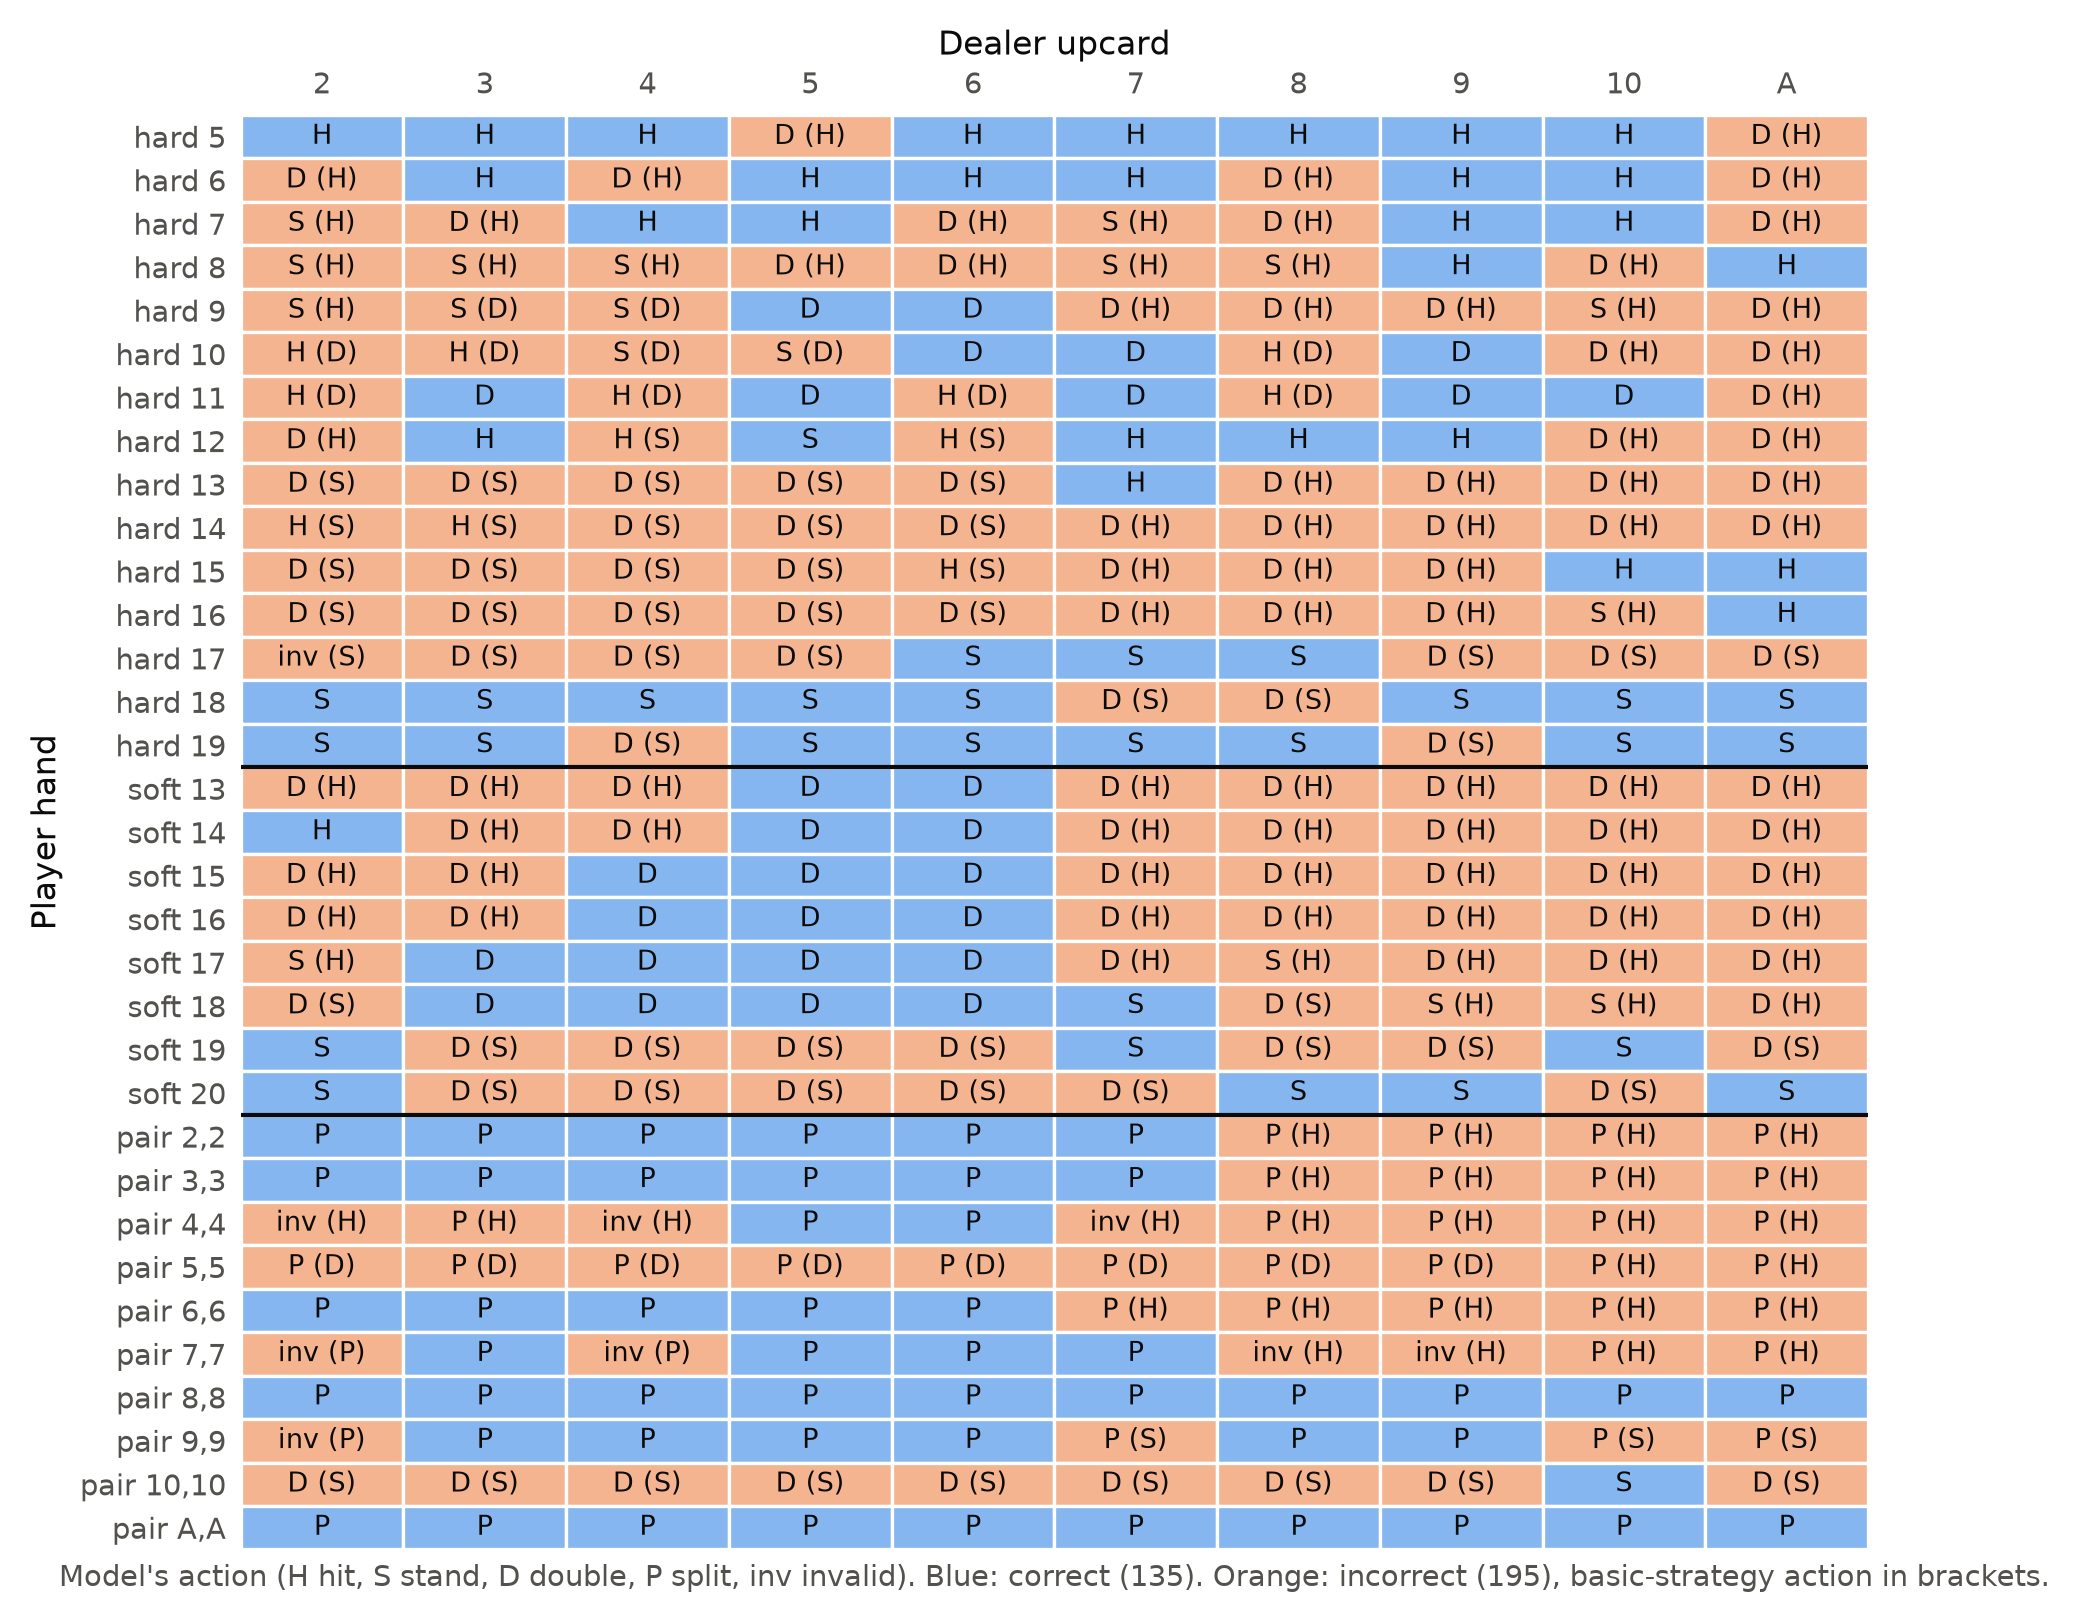
\includegraphics[width=\linewidth]{results/scenarios_seed2026/accuracy_heatmap.png}
  \caption{Scenario set: the model's action in each of the 330 basic-strategy
  cells (H hit, S stand, D double, P split). Blue cells are correct and orange
  cells are incorrect, with the correct action in brackets.}
  \Description{Heatmap of player hands (rows) against dealer upcards
  (columns), each cell labeled with the model's action and colored by whether
  it matches basic strategy.}
  \label{fig:scenario}
\end{figure}

\begin{figure}[t]
  \centering
  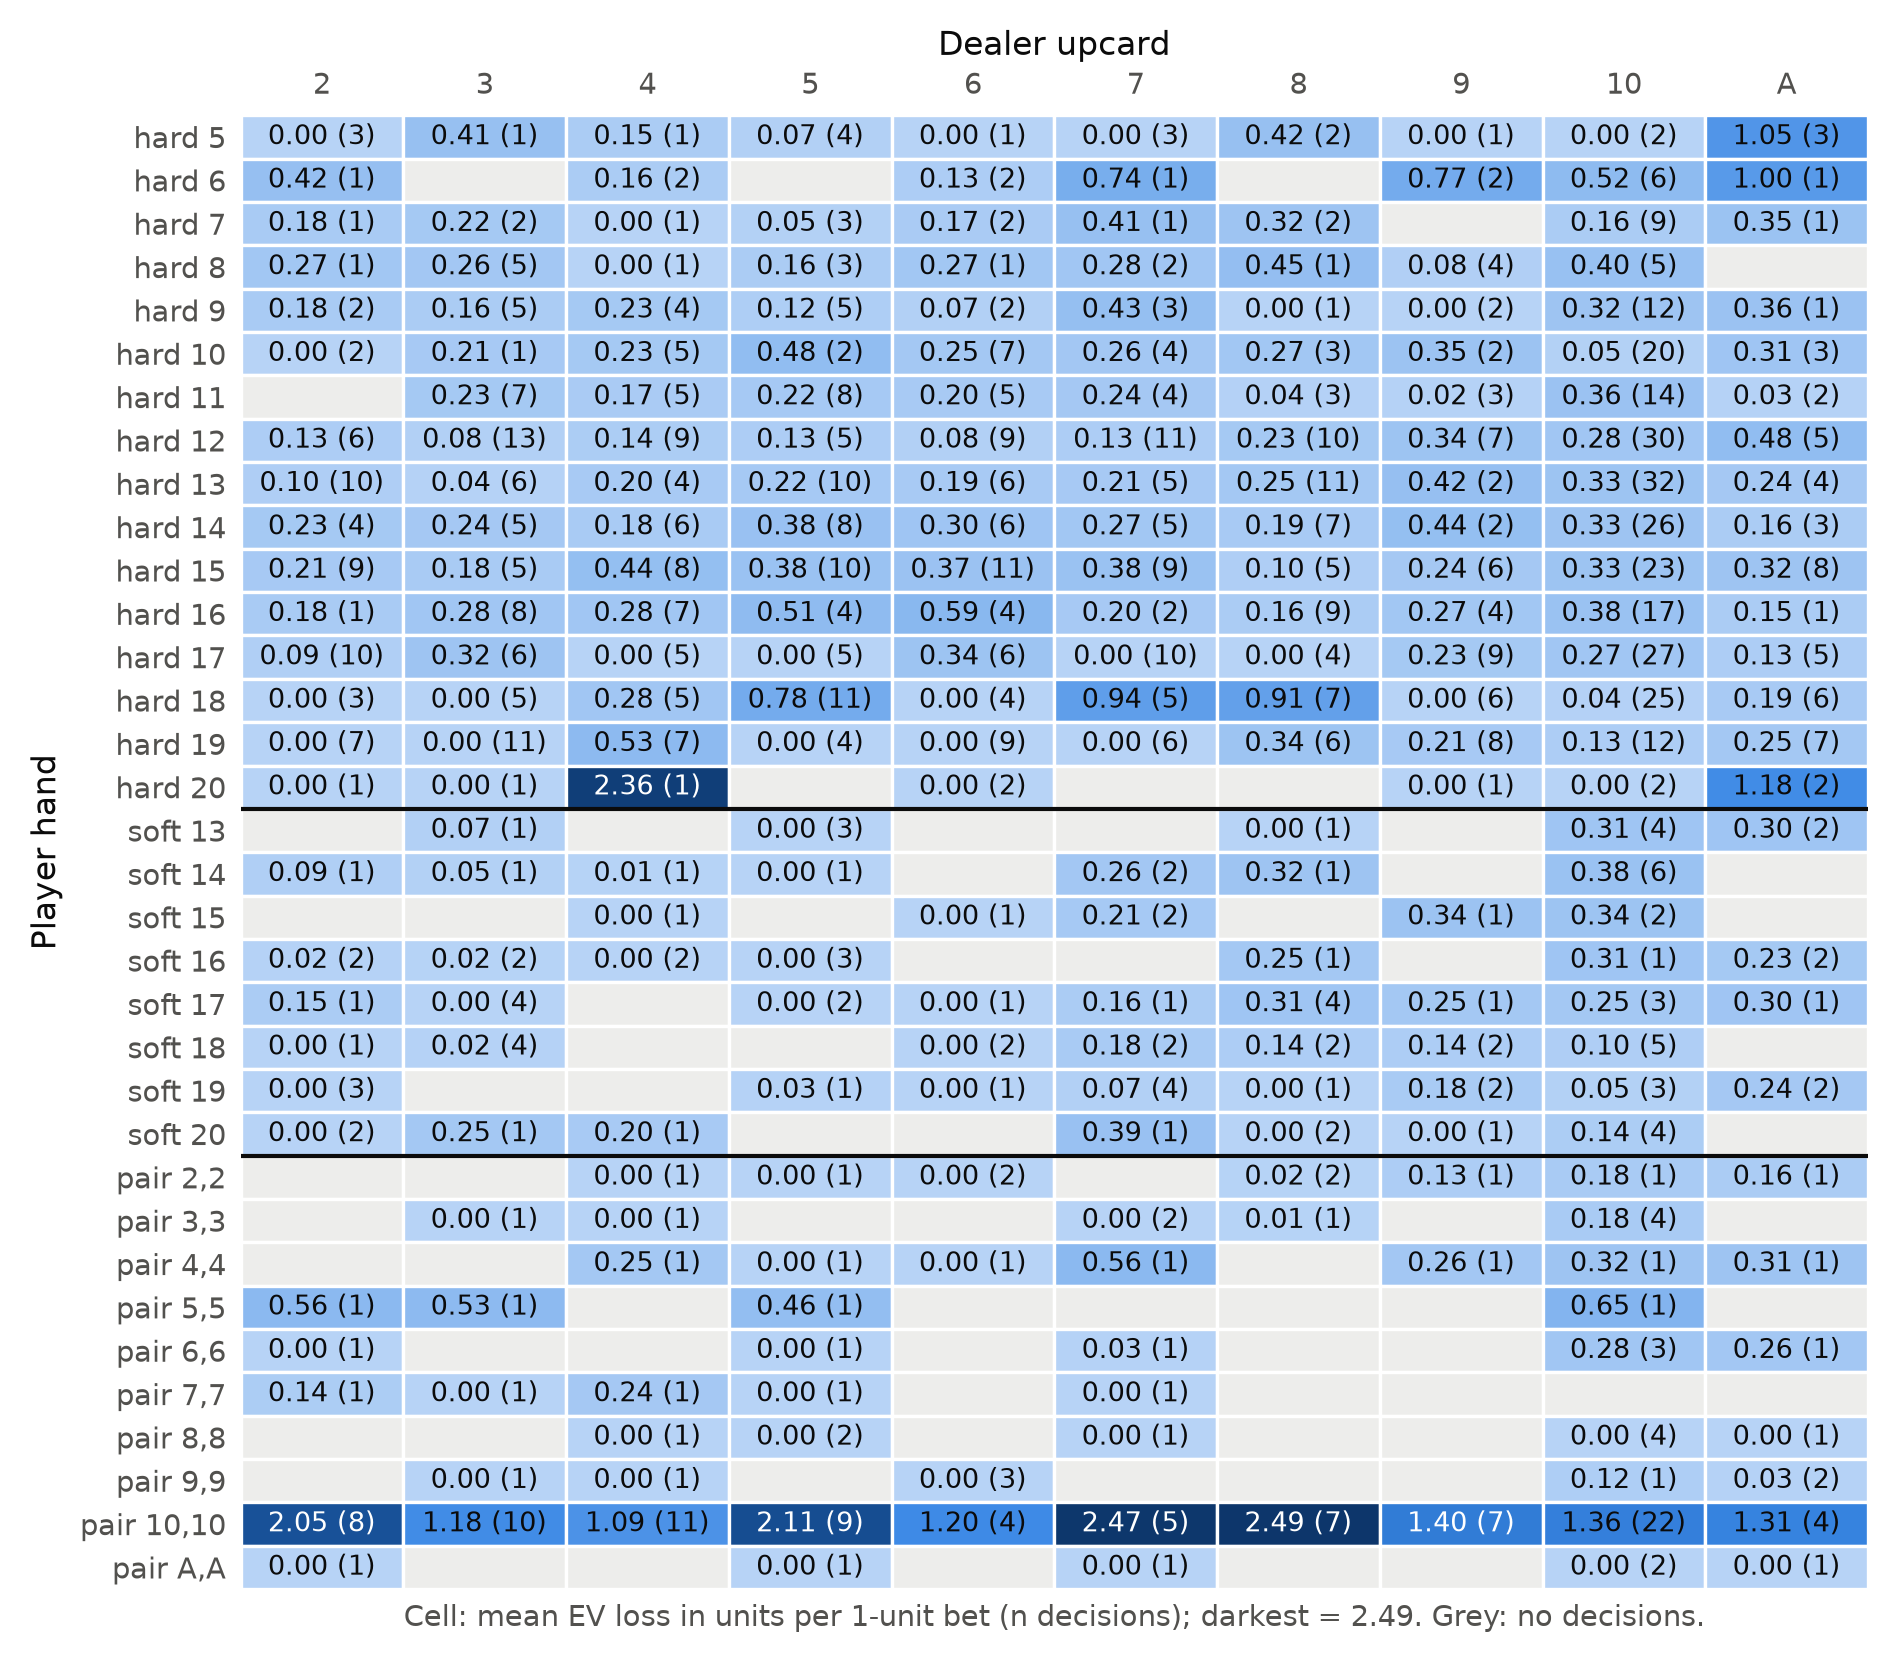
\includegraphics[width=\linewidth]{results/baseline_seed2026/ev_loss_heatmap.png}
  \caption{Natural run: mean EV loss per decision by player hand and dealer
  upcard. The 10,10 row, where the model often doubled instead of standing,
  dominates the loss.}
  \Description{Heatmap of mean expected-value loss per decision by player hand
  and dealer upcard; the row for a pair of tens is darkest.}
  \label{fig:evloss}
\end{figure}

% ---------- BibTeX: add to the .bib file ----------
% @online{wizardofodds,
%   author  = {Michael Shackleford},
%   title   = {4-8 Deck Blackjack Strategy},
%   organization = {Wizard of Odds},
%   url     = {https://wizardofodds.com/games/blackjack/strategy/4-decks/},
%   urldate = {2026-11-22}
% }
% @misc{qwen2024qwen25,
%   author  = {{Qwen Team}},
%   title   = {Qwen2.5 Technical Report},
%   year    = {2024},
%   eprint  = {2412.15115},
%   archivePrefix = {arXiv}
% }
